\documentclass[twocolumn]{article}
% Language setting
% Replace `english' with e.g. `spanish' to change the document language
\usepackage[spanish]{babel}
\addto{\captionsspanish}{\renewcommand{\abstractname}{Abstract}}
% Set page size and margins
% Replace `letterpaper' with `a4paper' for UK/EU standard size
\usepackage[letterpaper,top=2cm,bottom=2cm,left=3cm,right=3cm,marginparwidth=1.75cm]{geometry}

% Useful packages
\usepackage{amsmath}
\usepackage{cancel}
\usepackage{graphicx}
\usepackage[colorlinks=true, allcolors=blue]{hyperref}
\usepackage{blindtext}
\usepackage{multicol}
\usepackage{abstract}

\title{Regresión lineal para predicción de homicidios en Estados Unidos}
\author{José Pablo Martínez Valdivia}

\begin{document}

\twocolumn[
  \maketitle
  \begin{onecolabstract}
    Crime prediction is a problem that involves a huge amount social and environmental factors.
    This paper explores methods of data management and data processing and the
    barebones implementation of a linear regression algorithm trained by gradient descent.
    This regression aims to predict the number of murders in the United States of America
    using a set of social data from each state.
  \end{onecolabstract}
]

% \begin{keyword}
% asd
% \end{keyword}

\section{Introducción}
El dataset "Communities and Crime Unnormalized" fue conseguido del 
"UCI Machine Learning Repository" y consta de 125 variables y 2215 instancias
de datos poblacionales y de crímenes sucedidos entre 1990 y 1995. El objetivo 
del análisis es encontrar un modelo que pueda predecir la cantidad de homicidios.

\section{ETL}
\subsection{Extracción}
Los datos fueron descargados por medio de la librería de "ucimlrepo". Estos contienen 
datos poblacionales como:
\begin{itemize}
  \item Código de estado
  \item Cantidad de habitantes por estado
  \item Densidad poblacional
  \item Porcentaje de razas
  \item Cantidad de asesinatos
  \item Incendios provocados
  \item Asaltos
\end{itemize}
Entre otras. 

La mayoría de las columnas no tienen datos nulos, sin embargo, muchas columnas 
referentes a la fuerza policial se encuentran truncadas a 343 valores. Se decidió 
eliminar todas estas columnas, ya que borrar las filas sacrificaría la cantidad de 
datos para entrenar el modelo e imputar los datos con media puede producir sesgos o 
errores en el modelo.

\subsection{Transformación}
Solo la columna de \textit{Estado} contiene variables categóricas, pero se decidió
añadir al modelo, ya que se espera que diferentes estados tengan influencia en 
la taza de crímenes. Esto se hizo por medio de codificación buscando las siglas 
únicas de cada estado y asignándoles un número dependiendo de su orden (de 0 a n estados).

Las variables numéricas se encontraban en distintos rangos de valores por lo cual 
se implementó un escalador usando la técnica de \textit{z-scaling} donde se toma 
la media y desviación estándar de la distribución y se usan para escalar las variables 
transformando la distribución a una con media en 0 y desviación estándar de 1.

\begin{equation}
  z = \frac{x - \mu}{\sigma}
\end{equation}

\section{Regresión}
\subsection{Modelo lineal}
Para este modelo tomamos la suposición de una relación lineal entre las variables
más un sesgo.
\begin{equation}
  Y_i = \beta_0 + \beta_1x_1 + \beta_2x_2 + ... + \beta_px_p
\end{equation}

Lo cual podemos representar de forma matricial para poder implementar las predicciones 
de todos los datos como:

\begin{equation}
  \begin{bmatrix}
    \beta_0 \\
    \beta_1 \\
    \beta_2 \\
    \vdots  \\
    \beta_p
  \end{bmatrix}
  \begin{bmatrix}
    1 & x_{11} & x_{12} & ... & x_{1p} \\
    1 & x_{21} & x_{22} & ... & x_{2p} \\
    \vdots & \vdots & \vdots & \ddots & \vdots \\
    1 & x_{n1} & x_{n2} & ... & x_{np} \\
  \end{bmatrix}
  =
  \begin{bmatrix}
    y_1 \\
    y_2 \\
    \vdots  \\
    y_n
  \end{bmatrix}
\end{equation}

\subsection{Función de costo}
Se usó la función de \textit{Mean square Errors (MSE)} la cual representa el promedio
de las divergencias de la predicción y la variable esperada al cuadrado

\begin{equation}
  MSE = \frac{1}{n}\sum_{i = 1}^n (Y_i - \hat{Y})^2
\end{equation}

Usamos esta función para encontrar el error en los pesos y poder ajustar respectivamente
en un proceso iterativo.

\subsection{Descenso Gradiente}
Evaluando nuestra función de costo llámese \(J(\theta)\), con respecto a cada uno 
de los pesos \(\theta\) y multiplicando por un valor de aprendizaje \(\alpha\) 
podemos ajustar cada uno de los pesos de la siguiente manera.

\begin{equation}
  \theta := \theta - \alpha \frac{\partial}{\partial\theta}J(\theta)
\end{equation}

Realizando esto en un proceso iterativo, podemos llegar a un mínimo local de la 
ecuación y disminuir el error.

\subsection{Coeficiente de Determinación}
La \(R^2\) es una métrica que mide la variabilidad de un factor con respecto a otro.
Este lo obtenemos tomando 1 menos el cociente de la suma de las divergencias de 
la variable \(Y\) con sus predicciones \(\hat{Y}\) al cuadrado, sobre la suma
de sus diferencias con la media \(\bar{Y}\) al cuadrado.

\begin{equation}
  R^2 = 1 - \frac{\sum_{i=1}^{n} (Y_i - \hat{Y_i})^2}{\sum_{i=1}^{n} (Y_i - \bar{Y_i})^2}
\end{equation}

Este valor entre más cercano a uno nos indica que hay mayor probabilidad de que
la predicción explique a la variable objetivo. Esta métrica será usada más adelante 
para evaluar el modelo.

\subsection{Entrenamiento}
Las filas del dataset fueron aleatorizadas y separadas en tres conjuntos; 
entrenamiento, validación y prueba, estos constan del 60\%, 20\% y 20\% de los
datos respectivamente. Esta separación se hizo para garantizar la eficiencia 
del modelo ante datos nuevos y castigar el sobre ajuste que pueda tener al trabajar
solo con los datos provistos.

Posteriormente se corrió la regresión lineal con el descenso gradiente hasta que 
no hubiera cambio en los coeficientes o un número fijo de epochs se cumpliera. 
Cada epoch se calculo el \textit{MSE} tomando la pérdida con el conjunto de validación
y ajustando los coeficientes en magnitud del valor de aprendizaje.

\section{Resultados}
Después de 40,000 epochs, el modelo converge a un \textit{MSE} de 0.042171 y 
una \(R^2\) de 0.944747 comparando con el conjunto de prueba; esto representa un 
alto ajuste y poder predictivo del modelo con los datos reales de asesinatos en Estados unidos.
La figura [1] muestra la gráfica del error de la función de pérdida a través de las epochs.
Podemos ver que el modelo converge relativamente rápido y las 40000 están de más para el ajuste.

Finalmente podemos observar en la figura [2] como se comparan las predicciones con
los valores reales del conjunto de prueba. Se nota inicialmente que la predicción
se mantiene consistente para valores cercanos a 0 pero comienza a divergir con valores
de asesinatos más altos.

\begin{figure}
\centering
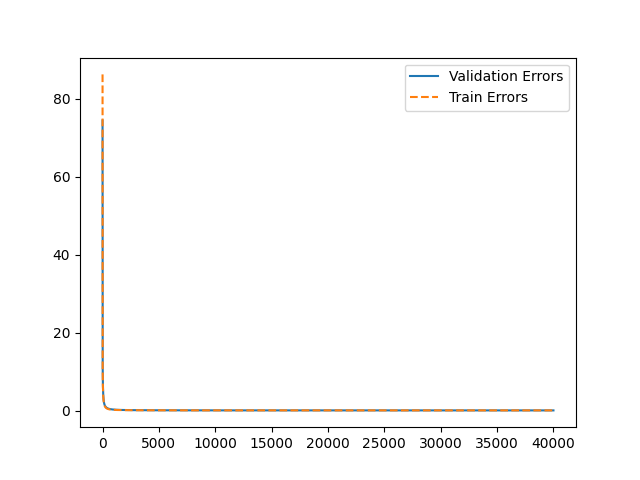
\includegraphics[width=0.4\textwidth]{assets/error.png}
\caption{\label{fig:dc1}Función de pérdida.}
\end{figure}

\begin{figure}
\centering
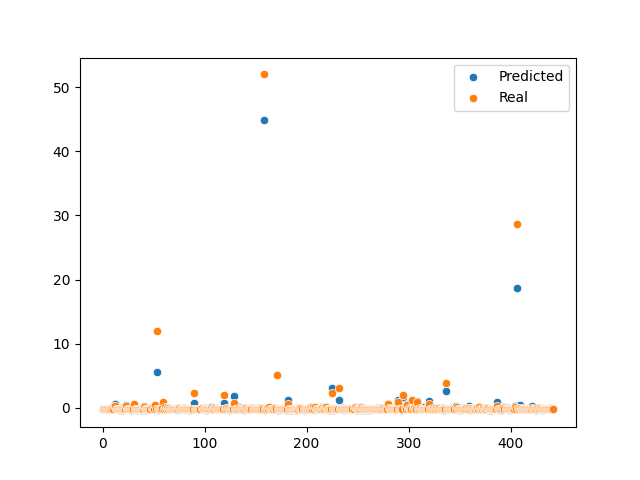
\includegraphics[width=0.4\textwidth]{assets/preds.png}
\caption{\label{fig:dc2}Resultado de la regresión.}
\end{figure}

\section*{Referencias}
Redmond,Michael. (2011). Communities and Crime Unnormalized. 
UCI Machine Learning Repository. https://doi.org/10.24432/C5PC8X.


\end{document}